\documentclass{standalone}
\usepackage{amsmath}
\usepackage[dvipsnames]{xcolor}
\usepackage{tikz} 
\usetikzlibrary{arrows, decorations.markings,decorations.pathreplacing,angles,quotes}
\usepackage{microtype}
\usepackage{fourier}

\definecolor{nblue}{RGB}{31, 119, 180}
\definecolor{py_olive}{rgb}{0.5, 0.5, 0}

\begin{document}

\begin{tikzpicture}
   		\node[anchor=south west,inner sep=0] (Bild) at (0,0) {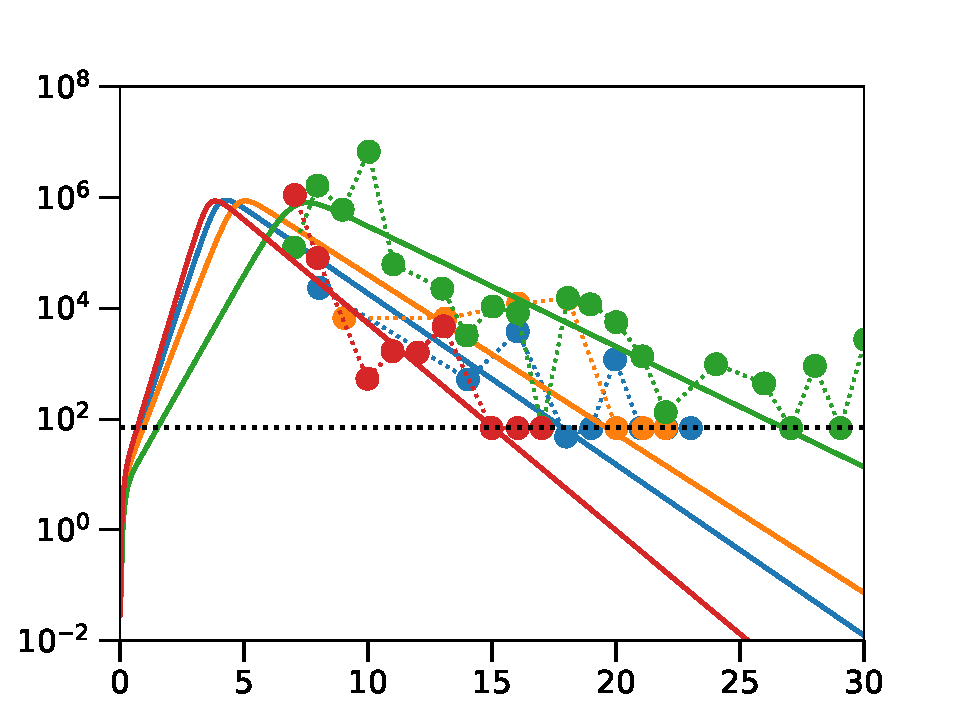
\includegraphics[scale=0.39]{fig1a_blank.pdf}};
   		\begin{scope}[x=(Bild.south east),y=(Bild.north west)]
			\node (right) at (1.5,0.5) {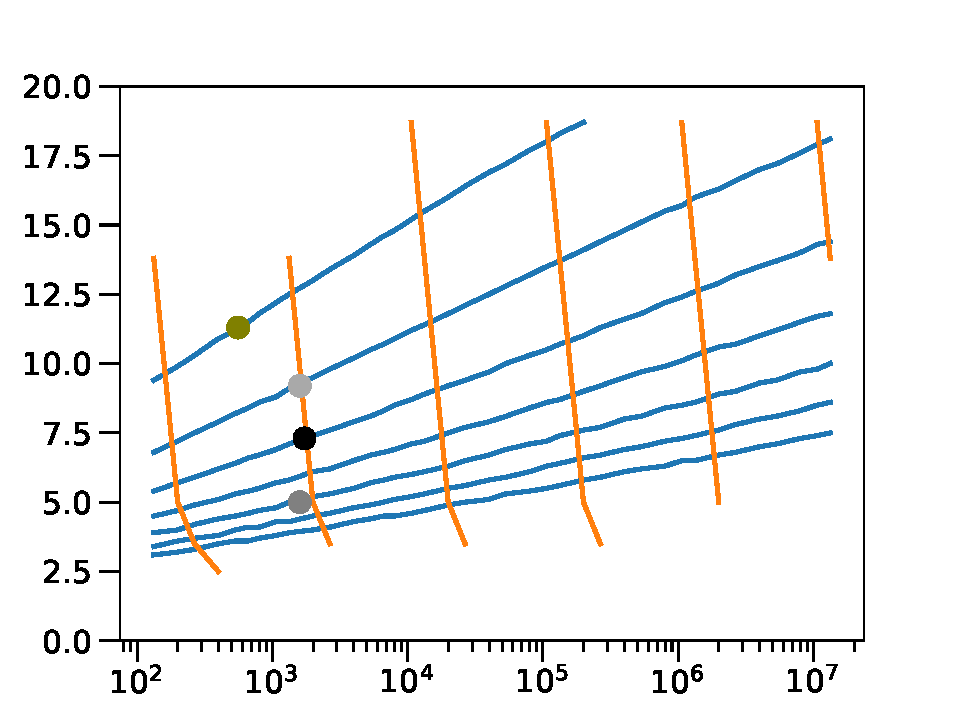
\includegraphics[scale=0.39]{fig1b_blank.pdf}};  
			  	
        	\draw (0.5,-0.035) node {time after infection (days)};
        	\draw (-0.015,0.5) node [rotate=90] {virus (copies.mL$^{-1}$)};   	
        	\draw (1.5,-0.035) node {proportion of susceptible target cells};
        	\draw (0.985,0.5) node [] {$R_0$};  
  	
        	\draw[black] (0.85,0.82) node {\Large \textbf{A}};
        	\draw[black] (1.175,0.82) node {\Large \textbf{B}};
        	
        	\draw[orange] (1.175,0.68) node {\tiny $10^5$};
			\draw[orange] (1.3,0.68) node {\tiny $10^6$};
        	\draw[orange] (1.4,0.82) node {\tiny $10^7$};
        	\draw[orange] (1.54,0.82) node {\tiny $10^8$};
        	\draw[orange] (1.68,0.82) node {\tiny $10^9$};
        	\draw[orange] (1.8,0.825) node {\tiny $10^{10}$};
        
        	\draw[nblue] (1.95,0.4) node {\tiny 9 days};
        	\draw[nblue] (1.95,0.44) node {\tiny 8 days};
        	\draw[nblue] (1.95,0.49) node {\tiny 7 days};
        	\draw[nblue] (1.95,0.56) node {\tiny 6 days};
        	\draw[nblue] (1.95,0.66) node {\tiny 5 days};
        	\draw[nblue] (1.95,0.8) node {\tiny 4 days};
        	\draw[nblue] (1.6,0.9) node {\tiny 3 days};

			\fill[black] (1.64,0.18) circle (.07cm);
			\draw (1.64,0.18) node[right= 2pt] {\tiny Young et al. (2020)}; 
			\fill[gray] (1.64,0.13) circle (.07cm);   
			\draw (1.64,0.13) node[right= 2pt] {\tiny W{\"o}lfel et al. (2020)}; 			
			\fill[gray,opacity=0.6] (1.64,0.23) circle (.07cm);             	
        	\draw (1.64,0.23) node[right= 2pt] {\tiny To et al. (2020)};
        	
        	\fill[py_olive] (1.64,0.28) circle (.07cm);             	
        	\draw (1.64,0.28) node[right= 2pt] {\tiny Kissler et al. (2020)};  
    		\end{scope}
\end{tikzpicture}

\end{document}